\input{/Users/fulingyue/Desktop/ChineseRef.tex}
\input{/Users/fulingyue/Desktop/CodeRefDef.tex}
\title{Linear Model}
\author{Fu Lingyue}
\date{\today}

\begin{document}
  \pagestyle{main}

\begin{center}
    \Huge
    \textbf{CS420 Machine Learning }
\end{center}

\begin{center}
    \par March 2020
    \par Author: Fu Lingyue  \\Mail: fulingyue@sjtu.edu.cn
\end{center}

\tableofcontents
\newpage

\section{Prequisitions}
\subsection{ML's Goal}
Machine learning has a loss function $\mathcal{L}$, 
and we have to let it take the minimum by learning the parameters of $f_\theta$.
$$ 
\mathrm{min} \{\frac{1}{N} \Sigma_{i = 1}^N \mathcal{L} (y_i,f_\theta(x_i))\}
$$

是预测结果接近真实的标签,是机器学习总体的目标。

\subsection{Outline of Proper Nouns}
\paragraph{欠拟合、过拟合}
算法无法捕捉数据基础变化趋势时,出现欠拟合;
模型把随机误差和噪声也考虑进去时,出现过拟合。

\paragraph{正则化(Regularization)} Add a parameter($\lambda \Omega(\theta)$) penalty to prevent the model from overfitting the data. Also in matrix form, it is to prevent singular matrices.

L2 regularization(Ridge): $\Omega(\theta) = ||\theta||^2_2 = \Sigma_{m=1}^M\theta_m^2$.

L1 regularization(Lasso): $\Omega(\theta) = ||\theta||_1 = \Sigma_{m=1}^M|\theta_m|.$

\begin{figure}[h]
  \begin{minipage}{0.48\linewidth}
    \centerline{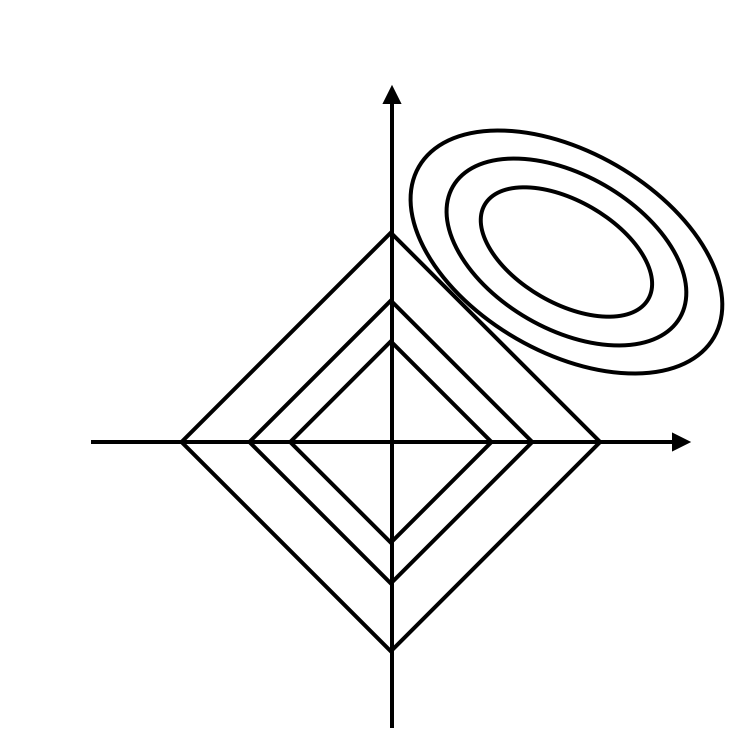
\includegraphics[width = 0.5\textwidth]{ref/L1}}
    \label{L1}
    \caption{L1 Reguraization}
  \end{minipage}
\hfill
\begin{minipage}{0.48\linewidth}
  \centerline{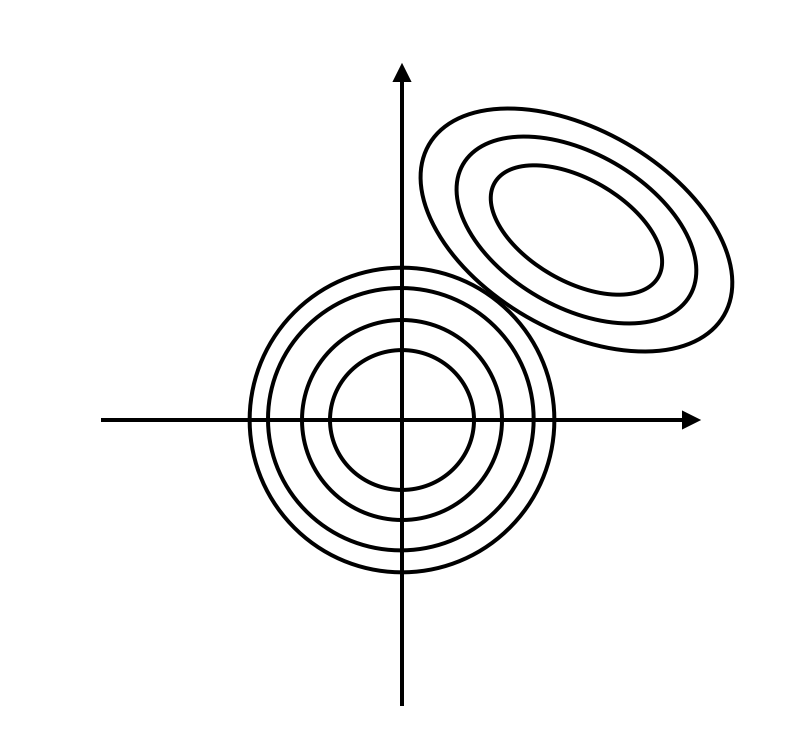
\includegraphics[width = 0.6\textwidth]{ref/L2}}
    \label{L2}
    \caption{L2 Reguraization}
\end{minipage}
\end{figure}

\paragraph{交叉验证(Cross Validation)} The training data were randomly divided into k groups, and every time we use one group to verify our model.


\paragraph{模型泛化性(Model Generalization)} 

\paragraph{判别模型和生成模型} 判别模型关注数据中的一维(显式函数);生成模型关注数据之间的联系(隐函数).

\paragraph{超参数} 模型运行前就根据经验选定的参数,它们只能够人工调整而不能通过学习得到,它们的选取会关系到模型学习的效率、结果、方向等等。
\subsection{分类指标}
有一类模型,我们用概率$p_\theta(y|x)$来描述它的预测值,叫\textbf{概率判别模型}。
而预测得到的概率,我们可以设置阈值来分类,包括二分类和多分类。

\section{线性判别模型(Linear Model)}
\paragraph{线性回归(Linear Regression)}
$$f(x) = \theta_0 + \theta_1x_1 + \theta_2x_2$$

(本节以\textbf{平方误差}$\mathcal L(y_i,f_\theta(x_i)) = \frac{1}{2}(y_i-f_\theta(x_i))^2$为例)

\paragraph{梯度下降方法 (Gradient Descent Algorithm)}
众所周知,梯度的方向是函数下降最快的方向。因此我们对于目标函数关于$\theta$ 取梯度,就可以得到它在$\theta$维度下降最快的方向,然后对$\theta$进行新的赋值:
$$\theta_\text{new} \leftarrow \theta_\text{old} - \eta\frac{\partial \mathcal L(\theta)}{\partial \theta}$$

这里的$\eta$ 是一个超参数,代表了梯度下降的步长。步长过长会导致越过最优点来回震荡,步长太短会导致收敛速度较慢。

\subsection{梯度更新方法}

\begin{enumerate}
  \item 批量梯度下降 :根据整个数据的梯度更新,准确但是慢;
  \item 随机梯度下降 :根据某个数据的梯度更新,快但不确定性多;
  \item 小批量梯度下降:用minibatch的梯度更新,较快,较准,易并行。
\end{enumerate}

\begin{lemma}
  凸优化目标函数具有唯一最小点。
  \label{lemma1}
\end{lemma}
Lemma\ref{lemma1} 应用在机器学习中,就意味着一个凸优化目标函数可以从不同的初始化参数最终学习到相同的最优值。
其中,(下)凸函数$f:\mathbb R^n \to \mathbb R$的定义为:$\textbf{dom }f$ 是凸集,并且
$$f(tx_1+(1-t)x_2)\leq tf(x_1) + (1-t)f(x_2)\quad \forall x_1,x_2 \in \textbf{dom}f, 0\leq t \leq 1.$$

\subsection{矩阵形式(Matrix Form)}
因为数据集很大,所以我们读入的时候很可能是一个矩阵,因此需要考虑矩阵形式。同时,矩阵形式也能够从另一个角度解释正则化。

\paragraph{训练数据矩阵}

\begin{equation}
\nonumber 
\text{特征值 } \mathbf{X} = 
\left[
\begin{array}{c}
  \mathbf{x}^1 \\
  \mathbf{x}^2 \\
  \dots \\
  \mathbf{x}^n
\end{array}
\right]
=
\left[
\begin{array}{c c c c}
  x_1^1 & x_2^1 & \dots & x_d^1\\
  x_1^2 & x_2^2 & \dots & x_d^2\\
  & \dots & & \\
  x_1^n & x_2^n & \dots & x_d^n\\
\end{array}
\right]
\end{equation}

参数 $\mathbf{\mu} = (\mu_1 \quad \mu_2 \dots \mu_d)^T$, 标签 $\mathbf{y} = (y_1\quad y_2 \dots y_n)^T$.

\paragraph{预测结果}
$\mathbf{\hat y = X\mu = (x^1\mu \quad x^2\mu \dots x^n\mu)}$

\paragraph{目标函数(Loss Function)}
$J\mathbf{(\mu) = \frac{1}{2}(y-\hat y)^T(y-\hat y) = \frac{1}{2}(y - X\mu)^T(y-X\mu)}$

为了取到目标函数的最小值,我们需要求梯度为$0$的$\mu$值,即
\begin{equation}
\nonumber
  \begin{aligned}
    \frac{\partial J(\mathbf{\mu})}{\partial \mathbf \mu} &
    = \frac{1}{2}\frac{\partial (\mathbf y^T\mathbf y -\mathbf \mu^T\mathbf X\mathbf y - \mathbf y\mathbf X\mathbf \mu +\mathbf \mu^T\mathbf X^T\mathbf X\mathbf \mu)}{\partial \mathbf \mu} \\
    & = \frac{1}{2}\frac{\partial (\mathbf y^T\mathbf y -2\mathbf \mu^T\mathbf X\mathbf y+\mathbf \mu^T\mathbf X^T\mathbf X\mathbf \mu)}{\partial \mathbf \mu} \\
    & = \frac{1}{2} \frac{\partial (-2\mathbf \mu^T\mathbf X\mathbf y+\mu^T\mathbf X^T\mathbf X\mathbf \mu)}{\partial \mathbf \mu} (\text{J 是数字})\\
    & = -\mathbf X\mathbf y - ((\mathbf X^T\mathbf X)+(\mathbf X^T\mathbf X)^T)\mathbf \mu\\
    & = -\mathbf X^T(\mathbf y - \mathbf X\mathbf \mu)  = 0
  \end{aligned}
\end{equation}

这里用到了矩阵求导法则(See Appendix A).接着求解方程:
$$-\mathbf X^T(\mathbf y-\mathbf X\mathbf \mu) = 0$$
$$\mathbf{X^TX\mu} = \mathbf{X^Ty}$$
$$\mathbf \mu =\mathbf{ (X^TX)^{-1}X^Ty}$$
至此我们得到了最优的$\mathbf \mu =\mathbf{ (X^TX)^{-1}X^Ty}$,注意这里的$\mathbf X$和$\mathbf X^T$不一定有逆矩阵,所以不能化简消去。同时,如果$\mathbf{X^TX}$ 是奇异矩阵,那么连$\mathbf{X^TX}$ 的逆矩阵都无法计算。因此,我们引入了正则化(正则化的第二个用处):
$$J(\mathbf \mu) = \frac{1}{2}(\mathbf y-\mathbf X\mathbf \mu)^T(\mathbf y - \mathbf X\mathbf \mu) + \frac{\lambda}{2}||\mathbf \mu||_2^2 $$

相似的可以得到梯度$\displaystyle \frac{J(\mathbf \mu)}{\mathbf \mu} = -\mathbf X^T(\mathbf y-\mathbf X\mathbf \mu) + \lambda \mathbf \mu$,
解出最优参数$\hat{\mathbf \mu} = (\mathbf X^T\mathbf X+\lambda\mathbf I)^{-1}\mathbf X^T\mathbf y$.

\subsection{泛线性模型}
泛线性模型是指,将给的特征映射到新的域上去,再用新的矩阵作为特征数据进行学习。它只是用了一个特征矩阵$\mathbf{\Phi_{n*h}}$(或者说是特征映射函数$\phi(x):\mathbb R^d \mapsto \mathbb R^h)$,进行了$x$到$\phi(x)$的转化。

类似的,我们有目标函数$J(\mathbf \theta) = \frac{1}{2}(\mathbf y-\mathbf X\mathbf \Phi\mathbf\theta)^T(\mathbf y - \mathbf X\mathbf\Phi\mathbf\theta)$, 梯度$\displaystyle \frac{\partial J(\mathbf \theta)}{\partial \mathbf \theta} = - \mathbf \Phi^T(\mathbf y - \mathbf X\mathbf \theta)$ 以及最优参数
以及最优参$\hat{\mathbf\theta} = \mathbf{(\Phi^T\Phi)^{-1}\Phi^T y}$.

引入$L2$正则化时,需要利用线性技巧来得到最优参数和预测值(略)。这里的K也被称为核矩阵,所以也叫\textbf{核线性回归}。

\subsection{逻辑回归(Logistic Regression)}
我们这里讨论的是概率判别模型,也就是用概率$p_\theta(y|x)$来描述某一类别的可能性。
\subsubsection{二分类}
\paragraph{概率特点} 只有$y=0$ 和$y=1$两种可能性,就有如下关系:
$$p_\theta(y=0|x) = 1-p_\theta(y=1|x)$$

而概率的大小则由一个sigmoid函数来决定,$\sigma(x) = \displaystyle\frac{1}{1+e^{-x}}$.
\begin{figure}[h]
  \centering
  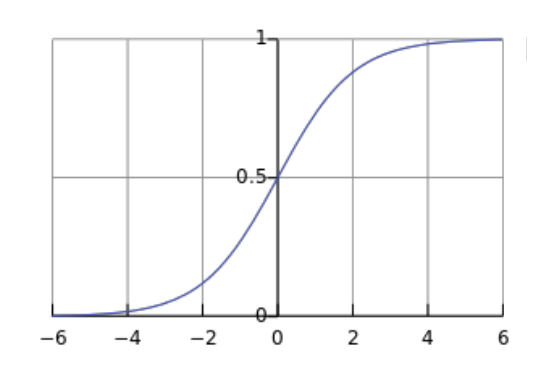
\includegraphics[width = 0.5\textwidth]{ref/sigmoid}
  
  \label{sigmoid}
  \caption{sigmoid函数}
\end{figure}

Sigmoid函数将一个数字映射到$(0,1)$区间里,我们把它看作是选择概率。
$$p_\theta(y=1|x) = \sigma(\theta^Tx) = \displaystyle\frac{1}{1+e^{-\theta^Tx}}$$
$$p_\theta(y=0|x) = 1 - \sigma(\theta^Tx) = \displaystyle\frac{e^{-\theta^Tx}}{1+e^{-\theta^Tx}}$$

选择sigmoid函数的原因是它不仅能够映射到(0,1),而且它有一个很好的性质:

$$\displaystyle \frac{\partial\sigma(z)}{\partial z} = \sigma(z)(1-\sigma(z))$$
\paragraph{损失函数——交叉熵函数}
$$H(p,q) = -\Sigma_xp(x)\log q(x)$$
$$H(p,q) = -\int_x\log q(x)\mathrm{d}x$$  
把二分类的概率特点代入后,得到
$$\mathcal L(y,x,p_\theta) = - y\log p_\theta(y=1|x) - (1-y)\log (1-p_\theta(y=1|x))$$
这就是二分类所使用的损失函数了。

\paragraph{梯度} 依然使用梯度下降法,通过求损失函数对于$\theta$求偏导来得到梯度方向:
\begin{equation}
\nonumber
  \begin{aligned}
    \displaystyle\frac{\partial \mathcal L(y,x,p_\theta)}{\partial \theta} 
    & = -y\frac{1}{\sigma(\theta^Tx)}\sigma(\theta^Tx)(1-\sigma(\theta^Tx))x - (1-y)\frac{-1}{1-\sigma(\theta^Tx)}\sigma(\theta^Tx)(1-\sigma(\theta^Tx))x \\
    &= -y(1-\sigma(\theta^Tx))x + (1-y)\sigma(\theta^Tx) x \\
    & = (\sigma(\theta^Tx)-y)x
  \end{aligned}
\end{equation}

得到梯度后,更新 $\theta = \theta + \lambda \frac{\partial \mathcal L}{\partial \theta}$
\paragraph{预测结果}
通过选择概率更大的标签,得到新的预测结果:
\begin{equation}
  \nonumber
  \hat y = 
  \begin{cases}
    1, & p_\theta(y=1|x)> h(=0.5) \\
    0, & \text{otherwise}
  \end{cases}
\end{equation}
\paragraph{迭代} 再用预测结果去和实际的标签比较,得到新的loss函数,再次求梯度,再次更新参数$\theta\cdots$

附录B里展示了这部分的函数代码。

\subsubsection{多分类}
\paragraph{预测$y=c_j$概率}

$$p_\theta(y=c_j|x) = \displaystyle \frac{e^{\theta_j^Tx}}{\Sigma_{k=1}^m e^{\theta_k^T x}} \quad \text{for} j = 1,2,\dots,m$$

在这里,Sigmoid函数变化成了Softmax函数,将预测结果$\{\theta_k^Tx\}$标准化.
\paragraph{多分类交叉熵}
$$\mathcal L(y,x,p_\theta) = -\Sigma_k \delta(y=c_k)\log p_\theta(y=c_k|x)$$
它的梯度为

\begin{equation}
\nonumber
  \begin{aligned}
    \displaystyle \frac{\partial\log p_\theta(y=c_j|x)}{\partial \theta_j} & = \frac{\partial}{\partial\theta_j}\log \frac{e^{\theta_j^Tx}}{\Sigma_{k=1}^me^{\theta_k^Tx}} \\
    &= x - \frac{\partial}{\partial\theta_j}\log \Sigma_{k=1}^m e^{\theta^T_kx} \\
    & = x - \frac{e^{\theta_j^Tx}}{\Sigma_{k=1}^m e^{\theta_k^T x}}x \\
    & = (1-p_\theta(y=c_j|x))x
  \end{aligned}
\end{equation}


\subsection{支持向量机}
通过找到最优决策边界来分类样本的方法。
\paragraph{最优决策边界}
每一个点都具有一定的噪音范围,当噪音范围变大的时候,划分边界变得越来越困难,而最优决策边界就是在噪音范围最大的情况下的那一条唯一的决策边界。

\begin{figure}[h]
\centering
  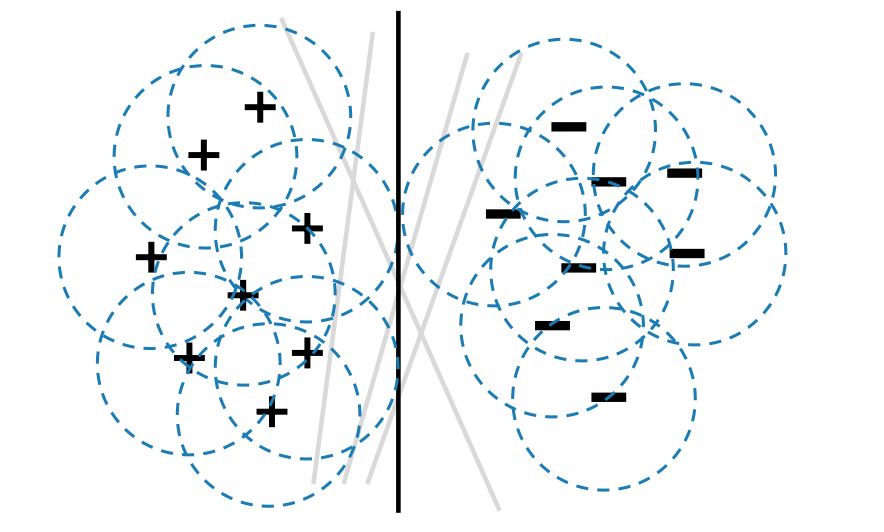
\includegraphics[width = 0.6\textwidth]{ref/border}
  \label{border}
  \caption{Optimal decision boundary}
\end{figure}

\subsubsection{打分函数}
打分函数和逻辑回归中的loss function 非常相似,其描述的是一个点与决策边界的距离。假设决策边界的方程为$\theta_0 + \theta_1x_1 + \theta_2x_2 = 0$,那么打分函数$s(x) = \theta_0 + \theta_1x_1 + \theta_2x_2$。打分函数的分数越高,样本离边界越远,我们的分界就有更高的置信度。


\subsubsection{标签预测}
经过支持向量机的计算过程后,我们会得到一个最优边界$(\omega,b)$,其中$\omega$是特征权重向量,$b$是截距。那么预测的结果就是$\omega^TX+b$,描述了$X$和我们最终得到的最有边界的距离。如果它大于0,说明在边界的右上区域,那么我们取标签为1,反之在左下区域,标签为-1,也就是函数
\begin{equation}
 \nonumber
    g(z) =
\begin{cases}
    +1 & z \geq 0 \\
    -1 & \text{otherwise.}
\end{cases}
\end{equation}

\subsubsection{最优边界的寻找}
在每一个给定边界$(\omega,b)$,每个样本都会有其对应的打分函数。
实际上,打分函数的值正比于该点到决策边界的垂直距离。当我们把打分函数乘上标签值,就可以去除正负的影响,得到一个完完全全正比于距离的打分函数。

*这里说“正比于”的 原因是,$(\omega,b)$等比缩放时并不会影响边界的位置,所以有可能是等于有可能是正比于。

我们假设$\omega$模长为1,那么$\gamma= y(\omega x+b)$就是距离了。在一个给定的训练集中,我们需要找到离边界最近的那个点,它的分数就是这个边界的得分,即$\gamma_{(\omega,b)} = \min \{\gamma_1,\gamma_2\dots \gamma_N\}$.

从整体上看,我们需要选择分数最高的那一个边界$(\omega,b)$,也就是$\max \{\gamma_{(\omega,b)}\}$.

因此我们得到了约束条件
$$y(\omega x + b) \geq \hat \gamma$$
在这个约束条件下,我们需要求
$$\max \frac{\hat\gamma}{||\omega||}$$

前面已经提到,$(\omega,b)$可以等比例缩放,所以我们可以改写一下约束条件和目标函数:
$$y(\omega x + b) \geq 1$$
$$\max \frac{1}{||\omega||}$$

这样会更好求解一些。

最后,为了可以用二次规划算法求解,我们把目标函数改写成$min \frac{1}{2}||\omega||^2$.

\subsubsection{支持向量机的一些优化}
众所周知,拉格朗日有一个函数是用来优化计算线性规划问题的。

当限制条件是等式的时候,我们假设约束条件为$h_i(w) = 0$,目标函数是$\min f(w)$. 那么定义拉格朗日函数$\mathcal L(w,\beta) = f(w) + \Sigma_{i=1}^l\beta_ih_i(w)$. 拉格朗日的定理表明,求解
$$\frac{\partial\mathcal L(w,\beta)}{\partial w} = 0,\quad \frac{\partial\mathcal L(w,\beta)}{\partial \beta} = 0$$
就可以得到问题的解。

而在不等式的情况下,引入



\newpage
\appendix

\section{矩阵求导法则}
\label{matrix gradient}
\begin{enumerate}
  \item $\partial (XY) = (\partial X)Y + X\partial Y$;
  \item $\partial (X^T) = (\partial X)^T;$
  \item $\partial X^{-1} = -X^{-1}(\partial X)X^{-1}$;
  \item $\partial X^T = (\partial X)^T$;
  \item $\displaystyle \frac{\partial x^T b}{\partial x} = \displaystyle\frac{\partial b^T x}{\partial x} = b$;
  \item $\displaystyle \frac{\partial a^TXb}{\partial X} = ab^T$;
  \item $\displaystyle \frac{\partial a^TXa}{\partial X} = \frac{\partial a^TX^Ta}{\partial X} = aa^T;$
  \item $\displaystyle \frac{\partial b^TX^TXc}{\partial X} = X(bc^T+cb^T)$;
  \item $\displaystyle \frac{\partial x^TBx}{\partial x} = (B+B^T)x$.
\end{enumerate}
\section{逻辑回归代码块}
\subsection{二分类}
\begin{lstlisting}
  def sigmoid(x):
        return 1.0 / (1 + np.exp(-x))
\end{lstlisting}
\begin{lstlisting}
  def l2_loss(self, X, Y, reg):
    mul = np.matmul(X,self.W)
    predict = sigmoid(mul)
    error =  predict - Y
    loss = - np.matmul(Y.T ,np.log(predict)) 
            - np.matmul((1 - Y).T, np.log(1-predict)) 
            + reg * np.matmul(W.T,W)/2 
    grad = np.matmul(X.T, error) + reg * self.W
    return loss, grad
\end{lstlisting}

\begin{lstlisting}
  def predict(self, X, threshold=0.5):
    mul = np.matmul(X,self.W)
    pre = sigmoid(mul)
    Y_pred = []
    for i in range(X.shape[0]):
      Y_pred.append(mul[i] > threshold)
    return Y_pred
\end{lstlisting}


\subsection{多分类}

\end{document}














